\chapter{Extracci� Contingut PDF}
\label{appendix-pdf2text}

A continuaci� es mostren exemples de com queden les cap�aleres d'alguns fitxers PDF a l'extreure-les en forma de text.

\section{Exemple 01}
\subsubsection{Estructura del PDF}
\begin{figure}[H]
\begin{center}
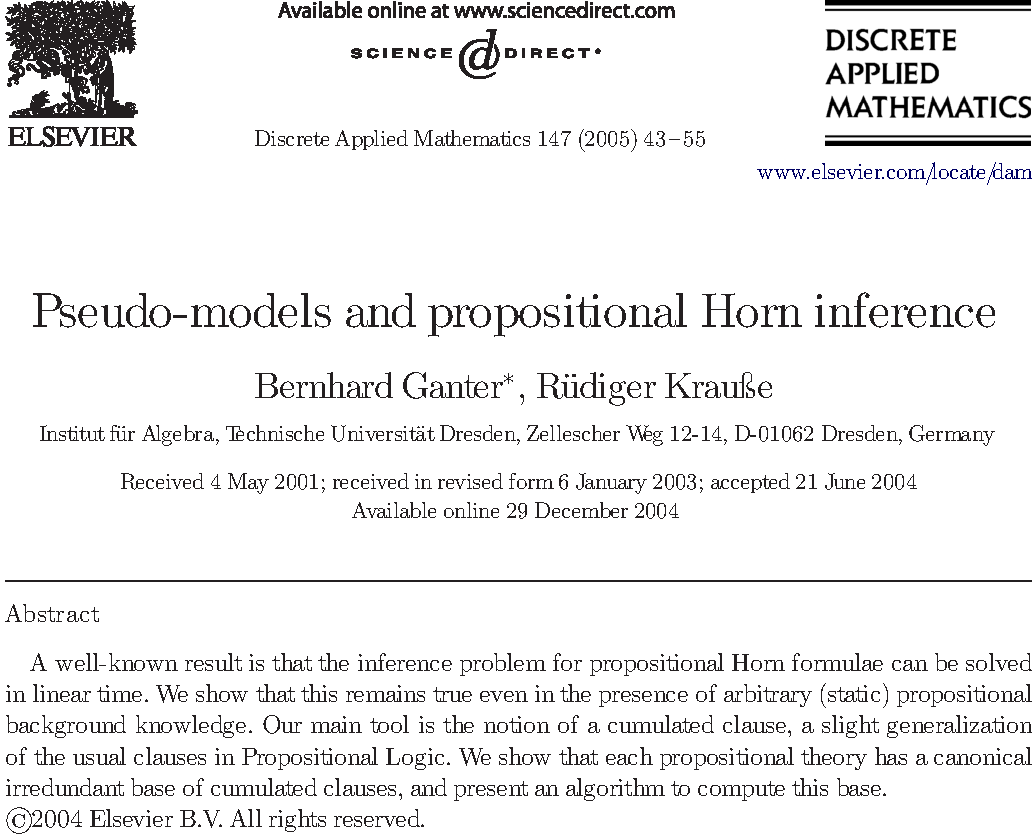
\includegraphics[width=0.85\textwidth]{figures/pdf2text/pdf2text:01.pdf}
%\caption{Primera idea per l'extracci� de refer�ncies}
\label{fig:pdf2text:01}
\end{center}
\end{figure}

\subsubsection{Text}
Discrete Applied Mathematics 147 (2005) 43 � 55 www.elsevier.com/locate/dam

Pseudo-models and propositional Horn inference
Bernhard Ganter , R�diger Krau�e
Institut f�r Algebra, Technische Universit�t Dresden, Zellescher Weg 12-14, D-01062 Dresden, Germany Received 4 May 2001; received in revised form 6 January 2003; accepted 21 June 2004 Available online 29 December 2004

Abstract A well-known result is that the inference problem for propositional Horn formulae can be solved in linear time. We show that this remains true even in the presence of arbitrary (static) propositional background knowledge. Our main tool is the notion of a cumulated clause, a slight generalization of the usual clauses in Propositional Logic. We show that each propositional theory has a canonical irredundant base of cumulated clauses, and present an algorithm to compute this base. � 2004 Elsevier B.V. All rights reserved.
MSC: 03B05; 03B35; 68T30 Keywords: Horn inference; Horn base; Background knowledge


\section{Exemple 02}
\subsubsection{Estructura del PDF}
\begin{figure}[H]
\begin{center}
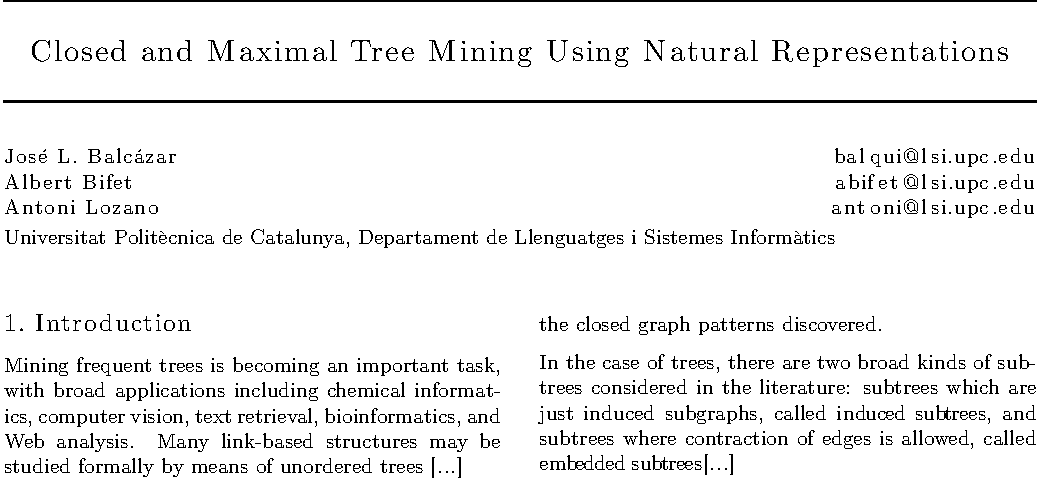
\includegraphics[width=0.85\textwidth]{figures/pdf2text/pdf2text:02.pdf}
\label{fig:pdf2text:02}
\end{center}
\end{figure}

\subsubsection{Text}
Closed and Maximal Tree Mining Using Natural Representations

Jos' L. Balc'zar e a balqui@lsi.upc.edu Albert Bifet abifet@lsi.upc.edu Antoni Lozano antoni@lsi.upc.edu Universitat Polit`cnica de Catalunya, Departament de Llenguatges i Sistemes Inform`tics e a

1. Introduction
Mining frequent trees is becoming an important task, with broad applications including chemical informatics, computer vision, text retrieval, bioinformatics, and Web analysis. Many link-based structures may be studied formally by means of unordered trees.


\section{Exemple 03}
\subsubsection{Estructura del PDF}
\begin{figure}[H]
\begin{center}

\includegraphics[width=0.85\textwidth]{figures/pdf2text/pdf2text:03.pdf}
\label{fig:pdf2text:03}
\end{center}
\end{figure}

\subsubsection{Text}
Applied Economics, 2010, 42, 825�850
\\
\\
Modelling the interactions across international stock, bond and foreign exchange markets\\
Abdul Hakima,* and Michael McAleerb\\
Department of Economics, University of Western Australia, Australia and Faculty of Economics, Indonesian Islamic University, Indonesia b Department of Economics, University of Western Australia, Australia
a
\\
\\
Downloaded By: [Consorci de Biblioteques Universitaries de Catalunya] At: 11:49 20 May 2010\\
\\
The benefits of investing internationally depend on three conditions, namely, cross-country correlations, market volatilities and future changes in currency risks (Odier and Solnik, 1993). This article investigates these conditions for several countries. Many papers have modelled [...]
